%%%%%%%%%%%%%%%%%%%%%%%%%%%%%%%%%%%%%%%%%%%%%%%%%%%%%%%%%%%%%%%%%%%%
\begin{frame}
\frametitle{Экономико-географического положение}

\begin{figure}[h!]
	\begin{center}
		{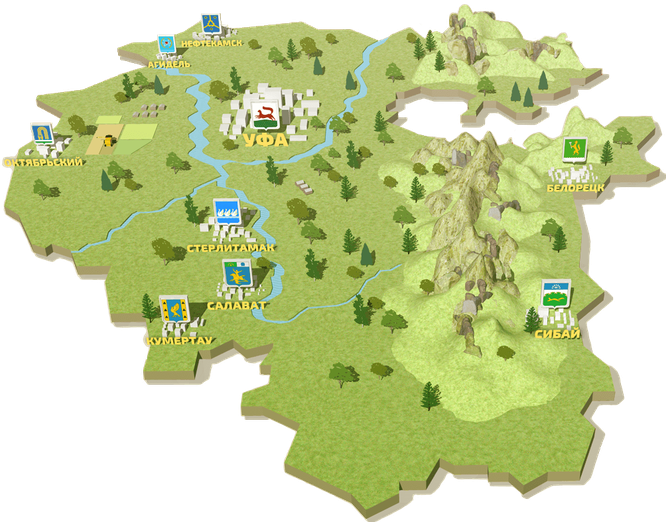
\includegraphics[width=85mm]{pics/alina/map.png}}
		\caption{Карта республики Башкортостан}
	\end{center}
\end{figure}

\end{frame}
%%%%%%%%%%%%%%%%%%%%%%%%%%%%%%%%%%%%%%%%%%%%%%%%%%%%%%%%%%%%%%%%%%%%

%%%%%%%%%%%%%%%%%%%%%%%%%%%%%%%%%%%%%%%%%%%%%%%%%%%%%%%%%%%%%%%%%%%%
\begin{frame}
\frametitle{Экономико-географического положение}

\begin{figure}[h!]
	\begin{center}
		{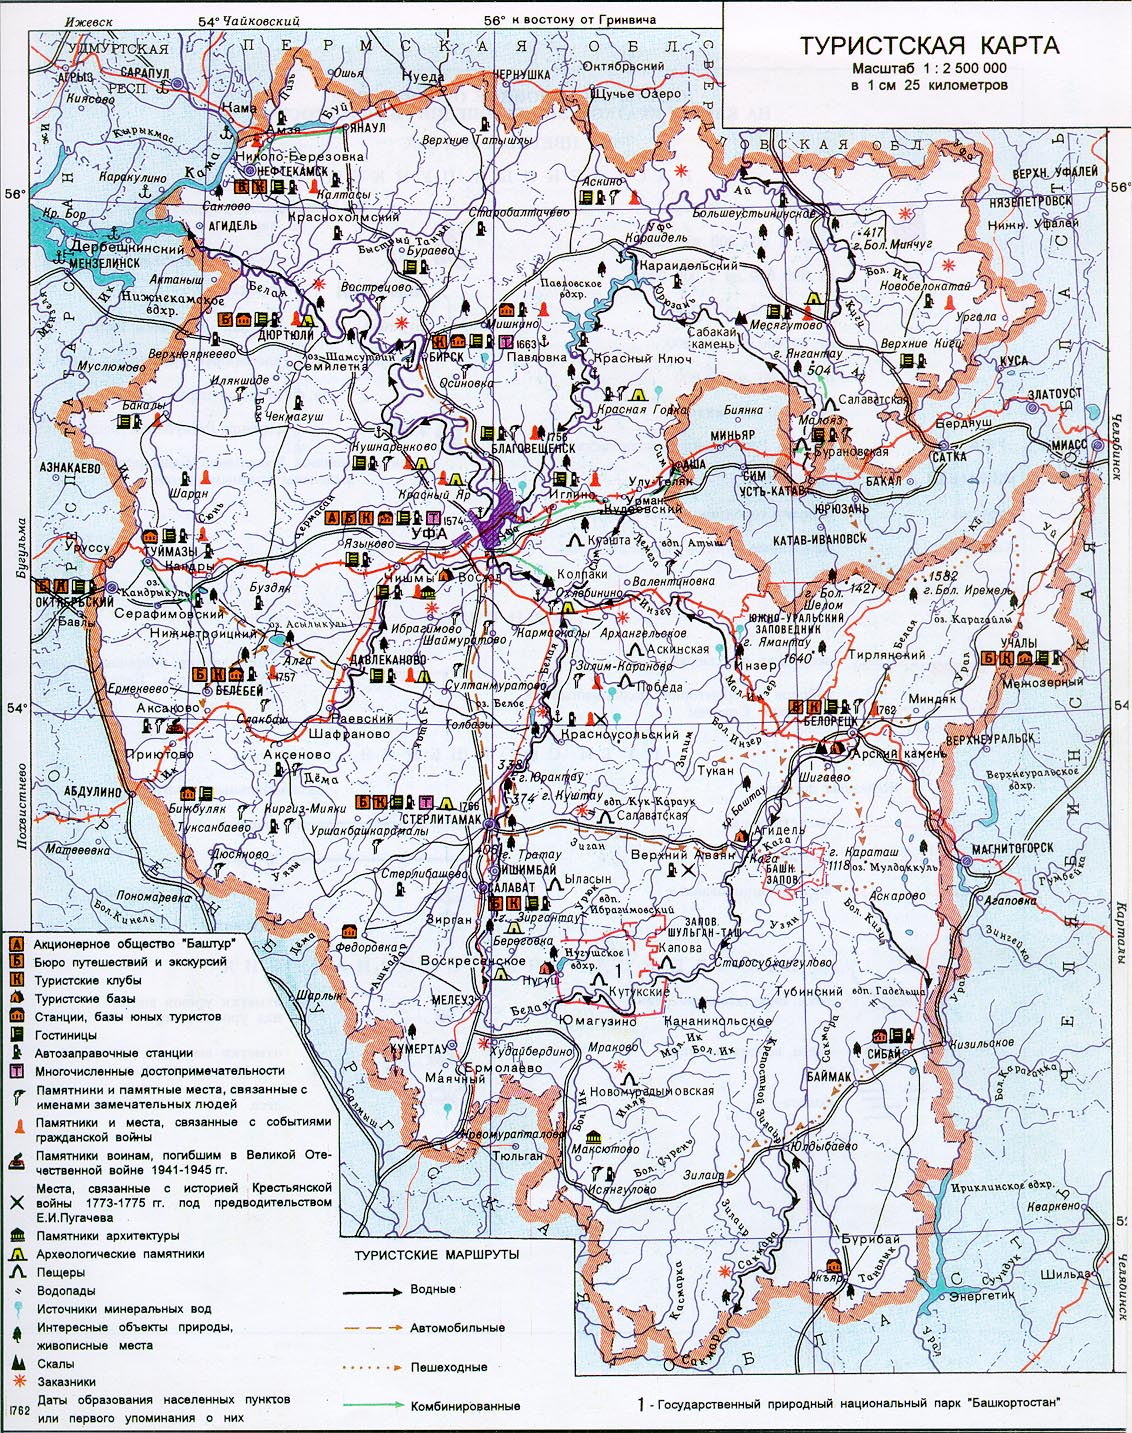
\includegraphics[width=60mm]{pics/alina/doroga.jpg}}
		\caption{Карта дорог республики Башкортостан}
	\end{center}
\end{figure}

\end{frame}
%%%%%%%%%%%%%%%%%%%%%%%%%%%%%%%%%%%%%%%%%%%%%%%%%%%%%%%%%%%%%%%%%%%%

%%%%%%%%%%%%%%%%%%%%%%%%%%%%%%%%%%%%%%%%%%%%%%%%%%%%%%%%%%%%%%%%%%%%
\begin{frame}
\frametitle{Экономико-географического положение}

\begin{figure}[h!]
	\begin{center}
		{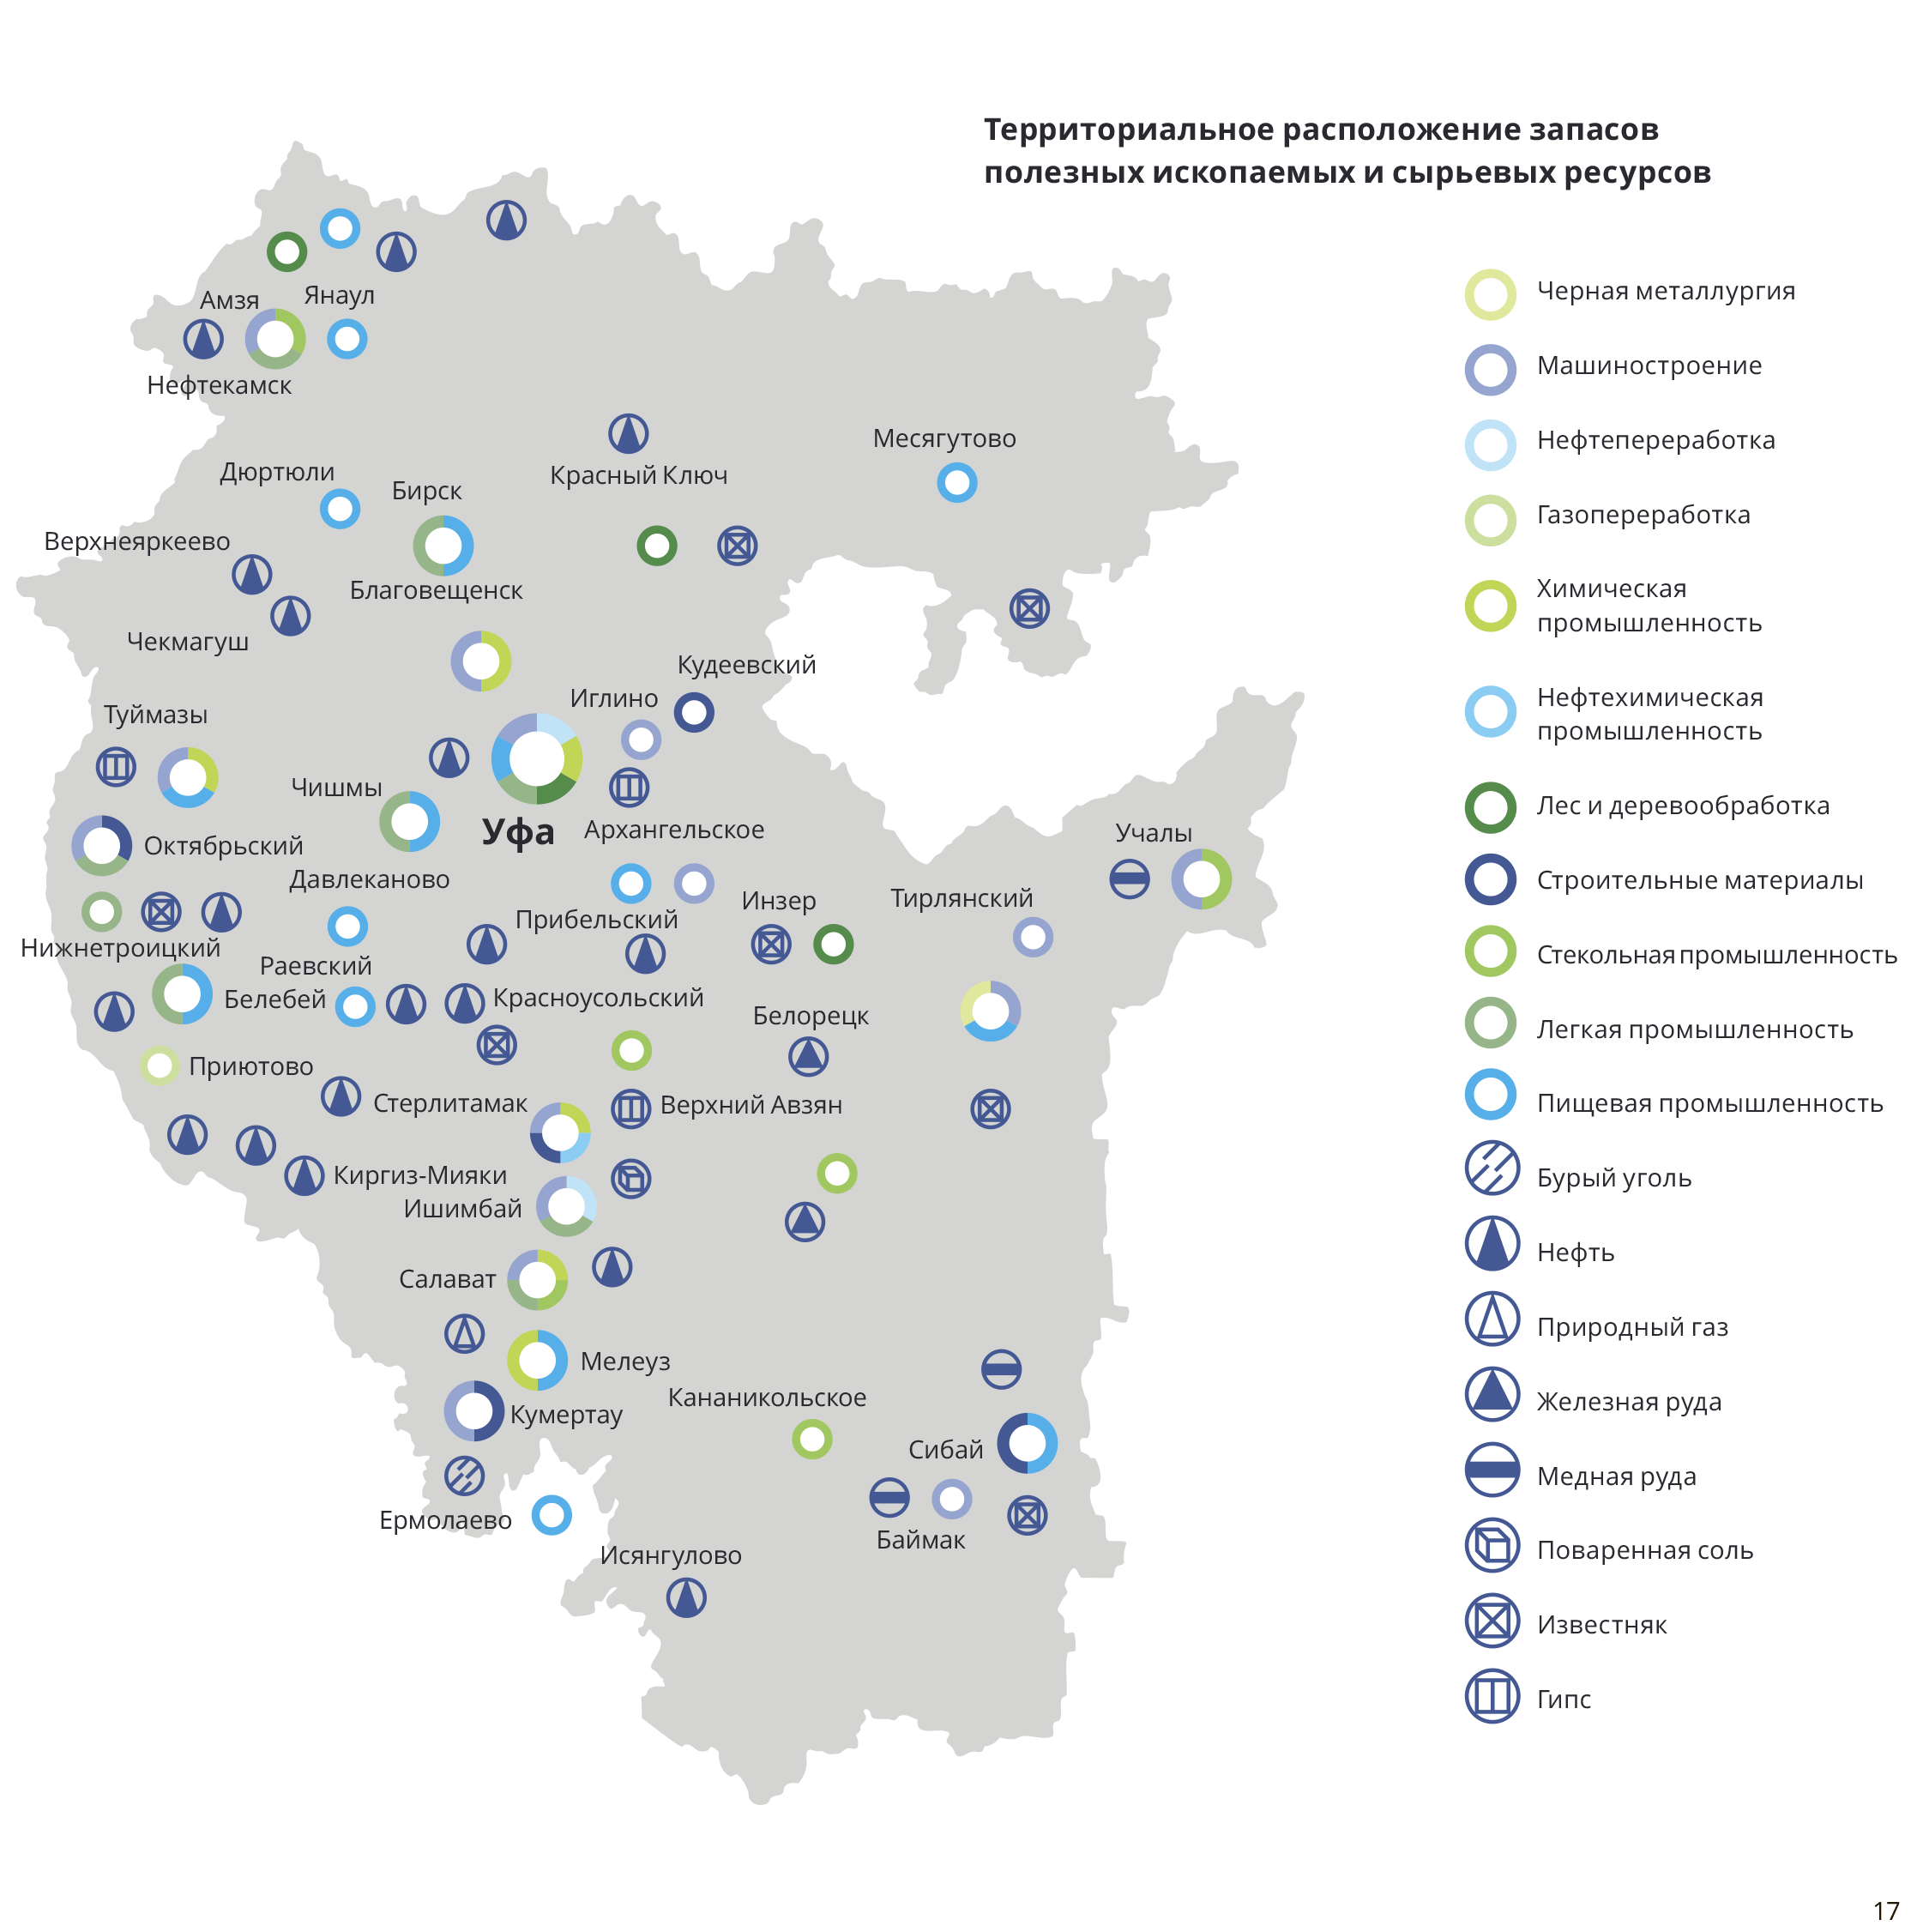
\includegraphics[width=85mm]{pics/alina/resource.png}}
	\end{center}
\end{figure}

\end{frame}
%%%%%%%%%%%%%%%%%%%%%%%%%%%%%%%%%%%%%%%%%%%%%%%%%%%%%%%%%%%%%%%%%%%%

%%%%%%%%%%%%%%%%%%%%%%%%%%%%%%%%%%%%%%%%%%%%%%%%%%%%%%%%%%%%%%%%%%%%
\begin{frame}
\frametitle{Административно-территориальная структура
	региона}

Современное административно-территориальное устройство Башкортостана регулируется Законом «Об административно-территориальном устройстве Республики Башкортостан» от 20 апреля 2005 года № 178-з. Во исполнение статьи 16 данного закона утверждён Реестр административно-территориальных единиц и населённых пунктов Республики Башкортостан.

\end{frame}
%%%%%%%%%%%%%%%%%%%%%%%%%%%%%%%%%%%%%%%%%%%%%%%%%%%%%%%%%%%%%%%%%%%%

%%%%%%%%%%%%%%%%%%%%%%%%%%%%%%%%%%%%%%%%%%%%%%%%%%%%%%%%%%%%%%%%%%%%
\begin{frame}
\frametitle{Административно-территориальная структура
	региона}

\begin{figure}[h!]
	\begin{center}
		{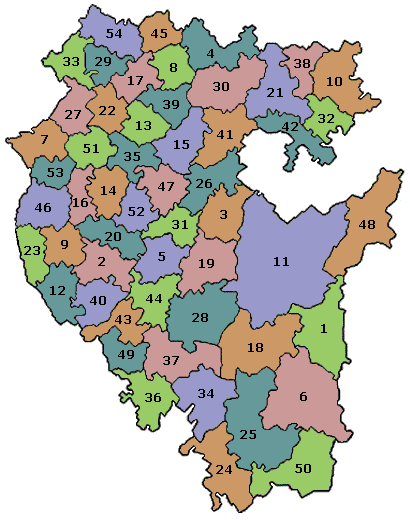
\includegraphics[width=50mm]{pics/alina/admin.png}}
		\caption{Районы Башкоростана}
	\end{center}
\end{figure}

\end{frame}
%%%%%%%%%%%%%%%%%%%%%%%%%%%%%%%%%%%%%%%%%%%%%%%%%%%%%%%%%%%%%%%%%%%%

%%%%%%%%%%%%%%%%%%%%%%%%%%%%%%%%%%%%%%%%%%%%%%%%%%%%%%%%%%%%%%%%%%%%
\begin{frame}
\frametitle{Административно-территориальная структура
	региона}

\begin{itemize}
	\item районы — 54
	\item внутригородские районы г. Уфы — 7
	\item рабочие посёлки (посёлки городского типа) — 2
	\item сельсоветы — 828
	\item сельские населенные пункты — 4538
\end{itemize}

\end{frame}
%%%%%%%%%%%%%%%%%%%%%%%%%%%%%%%%%%%%%%%%%%%%%%%%%%%%%%%%%%%%%%%%%%%%

%%%%%%%%%%%%%%%%%%%%%%%%%%%%%%%%%%%%%%%%%%%%%%%%%%%%%%%%%%%%%%%%%%%%
\begin{frame}
\frametitle{Административно-территориальная структура
	региона}

\begin{figure}[h!]
	\begin{center}
		{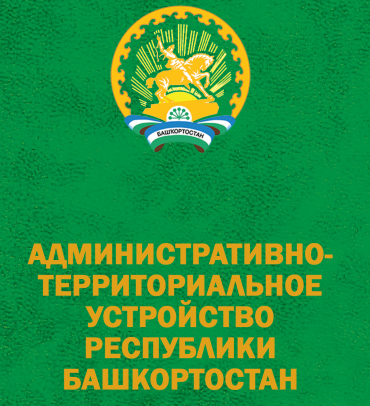
\includegraphics[width=55mm]{pics/alina/spravka.png}}
		\caption{Официальный справочник «Административно - территориальное устройство Республики Башкортостан»}
	\end{center}
\end{figure}

\end{frame}
%%%%%%%%%%%%%%%%%%%%%%%%%%%%%%%%%%%%%%%%%%%%%%%%%%%%%%%%%%%%%%%%%%%%
